%Präambel%
\documentclass[10pt]{scrartcl}
\usepackage[ngerman]{babel}
\usepackage[utf8]{inputenc}
\usepackage{graphicx}
\usepackage{amsmath}
\usepackage{amssymb}
\usepackage{xcolor,supertabular,multicol}
\usepackage{helvet}
\usepackage{lastpage}
\usepackage{geometry}
\usepackage{colortbl}
\usepackage{multirow}
\usepackage{color}
\usepackage{multicol}
\usepackage{wrapfig}
\usepackage{tipa} 
\makeatletter
\renewcommand*\env@matrix[1][*\c@MaxMatrixCols c]{%
  \hskip -\arraycolsep
  \let\@ifnextchar\new@ifnextchar
  \array{#1}}
\makeatother
\renewcommand{\familydefault}{\sfdefault}
%Kopfzeile%
\usepackage[headsepline, footsepline]{scrlayer-scrpage}
\pagestyle{scrheadings}
\clearpairofpagestyles
\setkomafont{pageheadfoot}{\normalfont\small}
\ihead{
\includegraphics[height=45pt]{images/HSRLOGO.jpg}}
\chead{}
\ohead{Zusammenfassung \\ Italienisch 1}
\ifoot{Züger Raphael \\ B16}
\cfoot{\today}
\ofoot{\pagemark /\pageref{LastPage}}
%Seitengeometrie festlegen%
\geometry{left=20mm, right=15mm, top=30mm, bottom=15mm, includefoot=false, headsep = \dimexpr2\baselineskip-5mm\relax, footskip = \dimexpr1\baselineskip+4mm\relax,}
%Fusszeitenlinie höher setzen%
\ModifyLayer[addvoffset=-.8ex]{scrheadings.foot.above.line}
\ModifyLayer[addvoffset=-.8ex]{plain.scrheadings.foot.above.line}
\setcounter{tocdepth}{2}
\usepackage{booktabs}			% Schönere Tabellen
\usepackage{tabularx}			% Tabellen auf Seitenbreite
\usepackage{enumitem} 
\newlist{citemize}{itemize}{4} 
\setlist[citemize]{label=\textbullet ,nosep,topsep=-\parskip} 
%Tabellen///////////////////////////////////////////////////%
\newcolumntype{L}[1]{>{\raggedright\arraybackslash}p{#1}} % Tabelleninhalt linksausgerichtet
\newcolumntype{R}[1]{>{\raggedleft\arraybackslash}p{#1}} % Tabelleninhalt rechtsausgerichtet
\newcolumntype{C}[1]{>{\centering\arraybackslash}p{#1}} %  Tabelleninhalt zentriert
\setlength{\parindent}{0pt}
\setlength{\columnsep}{1cm}
\newcount\n
\n=0
\def\tablebody{}
\makeatletter
\loop\ifnum\n<300
        \advance\n by1
        \protected@edef\tablebody{\tablebody
                \textbf{\number\n.}&
                \hfill T\hfill\hfill F\hfill\hskip0pt\endgraf
                \vskip.5\baselineskip
                \color@begingroup
                \color{black!20}
                \hrule height3ex
                \color@endgroup
                \tabularnewline
        }
\repeat
\makeatother

\begin{document}
\section*{Zusammenfassung Italienisch 1}
\begin{multicols*}{2}
\let\mcnewpage=\newpage
\makeatletter
\renewcommand\newpage{%
        \if@firstcolumn
                \hrule width\linewidth height0pt
                \columnbreak
        \else
                \mcnewpage
        \fi
}
\makeatother


\subsubsection*{Vokabular Unità 1}
\begin{supertabular}{p{4cm}p{4cm}}
\textbf{Saluti} & \textbf{Grussformel} \\ 
\\
a dopo & bis dann \\  
a presto & bis bald\\
arrivederci & auf Wiedersehen (formal)\\
buonanotte & gute Nacht\\
buonasera & guten Abend (formal)\\
buongiorno & guten Tag (formal)\\
ciao & Hallo / Tschüss (informell)\\
salve & Hallo / Servus (informell)\\
\\
\textbf{Primi contatti} & \textbf{Erste Kontakte}\\
\\
piacere & Angenehm!\\
\\
\textbf{In classe} & \textbf{In der Klasse}\\
\\
agenda \hfill f. & Kalender\\
cellulare \hfill m. & Handy\\
classe \hfill f. & Klassenzimmer\\
computer \hfill m. & Computer\\
evidenziatore \hfill m. & Leuchtstift\\
fotocopia \hfill f. & Fotokopie\\
gomma \hfill f. & Radiergummi\\
lavagna \hfill f. & Tafel\\
libro \hfill m. & Buch\\
matita \hfill f. & Bleistift\\
penna \hfill f. & Kugelschreiber\\
quaderno m. \hfill & Heft\\
scotch \hfill m. & Klebeband\\
sedia \hfill f. & Stuhl\\
tavolo \hfill m. & Tisch\\
vocabolario \hfill m. & Wörterbuch\\
zaino \hfill m. & Rucksack\\
\end{supertabular}
\subsubsection*{Vokabular Unità 2}
\begin{supertabular}{p{4cm}p{4cm}}
\textbf{Documenti in Italia} & \textbf{Ausweise in Intalien} \\ 
\\
carta d'identità \hfill f. & Personalausweis\\
passaporto \hfill m. & Passport\\
patente \hfill f. & Führerschein\\
tessera sanitaria \hfill f. & Versichertenkarte\\
\\
\textbf{Primi contatti} & \textbf{Erste Kontakte} \\
\\
chiocciola \hfill f. & At - Zeichen\\
cognome \hfill m. & Nachname\\
data \hfill f. & Datum\\
età \hfill f. & Alter\\
indirizzo e-mail \hfill m. & E-Mail Adresse\\
lingua \hfill f. & Sprache\\
nazionalità \hfill f. & Staatsbürgerschaft\\
nome \hfill m. & Vorname\\
numero di cellulare \hfill m. & Handynummer\\
numero di telefono  \hfill m. & Telefonnummer\\
professione \hfill f. & Beruf\\
punto \hfill m. & Punkt\\
trattino \hfill m. & Bindestrich\\
trattiono basso \hfill m. & Understrich\\
\\
\textbf{Nazionalità} & \textbf{Nationalitäten} \\
\\
americano /a & aus den USA\\
austriaco /a & Österreicher /in\\
cinese & Chinese / Chinesin\\
francese & Franzose / Französin\\
giapponese & Japaner /in\\
inglese & Engländer /in\\
italiano /a & Italiener /in\\
russo /a & Russe / Russin\\
spagnolo /a & Spanier /in\\
svizzero /a & Schweizer /in\\
tedesco /a & Deutscher / Deutsche\\
\\
\textbf{Professioni} & \textbf{Berufe} \\
\\
architetto /a \hfill m./f. & Architekt /in\\
attore \hfill m. & Schauspieler\\
attrice \hfill f. & Schauspielerin\\
avvocato /a \hfill m./f. & Rechtsanwalt /in\\
cameriere /a \hfill m./f. & Kellner /in\\
commesso / a \hfill m./f. & Verkäufer /in\\
dentista \hfill m./f. & Zahnarzt / Zahnärztin\\
fotografo /a \hfill m./f. & Fotograf /in\\
giornalista \hfill m./f. & Journalist /in\\
impiegato /a \hfill m./f. & Angestellte\\
imprenditore \hfill m. & Unternehmer\\
imprenditrice \hfill f. & Unternehmerin\\
ingegnere /a \hfill m./f. & Ingenieur /in\\
insegnante \hfill m./f. & Lehrer /in\\
medico /a \hfill m./f. & Arzt / Ärztin\\
poliziotto /a \hfill m./f. & Polizist /in\\
scienziato /a \hfill m./f. & Wissenschaftler /in\\
scrittore \hfill m. & Schriftsteller\\
scrittrice \hfill f. & Schriftstellerin\\
studente \hfill m. & Student\\
studentessa \hfill f. & Studentin\\
tassista \hfill m./f. & Taxifahrer /in\\
\\
\textbf{Luoghi di lavoro} & \textbf{Arbeitsorte} \\
\\
agenzia \hfill f. & Agentur\\
albergo \hfill m. & Hotel\\
banca \hfill f. & Bank\\
negozio \hfill m. & Geschäft / Laden\\
ristorante \hfill m. & Restaurant\\
scuola \hfill f. & Schule\\
studio fotografico \hfill m. & Fotostudio\\
\\
\textbf{Fare domande} & \textbf{Fragen stellen} \\
\\
che cosa? & was?\\
come? & wie?\\
di dove? & woher?\\
dove? & wo?\\
qual? & welche/r?\\
chi? & wer?\\
\\
\textbf{Numeri fino al 100} & \textbf{Zahlen bis 100} \\
\\
0 & zero\\
1 & uno\\
2 & due\\
3 & tre\\
4 & quattro\\
5 & cinque\\
6 & sei\\
7 & sette\\
8 & otto\\
9 & nove\\
10 & dieci\\
11 & undici\\
12 & dodici\\
13 & tredici\\
14 & quattordici\\
15 & quindici\\
16 & sedici\\
17 & diciasette\\
18 & diciotto\\
19 & diciannove\\
20 & venti\\
21 & ventuno\\
22 & ventidue\\
23 & ventitré\\
24 & ventiquattro\\
25 & venticinque\\
26 & ventisei\\
27 & ventisette\\
28 & ventotto\\
29 & ventinove\\
30 & trenta\\
31 & trentuno\\
32 & trentadue\\
33 & trentatré\\
34 & trentaquattro\\
35 & trentacinque\\
36 & trentasei\\
37 & trentasette\\
38 & trentotto\\
39 & trentanove\\
40 & quaranta\\
41 & quarantuno\\
42 & quarantadue\\
43 & quarantatré\\
44 & quarantaquattro\\
45 & quarantacinque\\
46 & quarantasei\\
47 & quarantasette\\
48 & qaurantotto\\
49 & quarantanove\\
50 & cinquanta\\
51 & cinquantuno\\
52 & cinquantadue\\
53 & cinquantatré\\
54 & cinquantaquattro\\
55 & cinquantacinque\\
56 & cinquantasei\\
57 & cinquantasette\\
58 & cinquantotto\\
59 & cinquantanove\\
60 & sessanta\\
61 & sessantuno\\
62 & sessantadue\\
63 & sessantatré\\
64 & sessantaquattro\\
65 & sessantacinque\\
66 & sessantasei\\
67 & sessantasette\\
68 & sessantotto\\
69 & sessantanove\\
70 & settanta\\
71 & settantuno\\
72 & settantadue\\
73 & settantatré\\
74 & settantaquattro\\
75 & settantacinque\\
76 & settantasei\\
77 & settantasette\\
78 & settantotto\\
79 & settantanove\\
80 & ottanta\\
81 & ottantuno\\
82 & ottantadue\\
83 & ottantatré\\
84 & ottantaquattro\\
85 & ottantacinque\\
86 & ottantasei\\
87 & ottantasette\\
88 & ottantotto\\
89 & ottantanove\\
90 & novanta\\
91 & cinquantuno\\
92 & novantadue\\
93 & novantatré\\
94 & novantaquattro\\
95 & novantacinque\\
96 & novantasei\\
97 & novantasette\\
98 & novantotto\\
99 & novantanove\\
100 & cento\\
\\
\textbf{All'università} & \textbf{An der universität} \\
\\
studio \hfill m. & Studium\\
facoltà \hfill f. & Fakultät\\
laurea triennale \hfill f. & Bachelor\\
laurea magistrale \hfill f. & Master\\
borsa di studio \hfill f. & Stipendium\\
frequentare & besuchen\\
studiare & studieren, lernen\\
\\
\textbf{Facoltà alla HSR} & \textbf{HSR - Studienrichtungen} \\
\\
Architettura del paesaggio \hfill f. & Landschaftsarchitektur\\
Elettrotecnica \hfill f. & Elektrotechnik\\
Energie rinnovabili e tecnica ambientale \hfill f. & Erneuerbare Energien und Umwelttechnik\\
Informatica \hfill f. & informatik\\
Ingegneria civile \hfill f. & Bauingenieurwesen\\
Ingegneria gestionale \hfill f. & Wirtschaftsingenieurwesen\\
Ingegneria meccanica / Innovazione \hfill f. & Maschinentechnik / Innovation\\
Pianificazione territoriale \hfill f. & Raumplanung\\
\end{supertabular}
\subsubsection*{Vokabular Unità Bonus A}
\begin{supertabular}{p{4cm}p{4cm}}
\textbf{I verbi giusti al bar e a colazione} & \textbf{Die passenden Verben in der Cafeteria und zum Frühstück} \\
\\
avere fame & hungrig sein\\
avere sete & durstig sein\\
bere & trinken\\
fare colazione & frühstücken\\
mangiare & essen\\
preferire & bevorzugen\\
prendere & nehmen\\
\\
\textbf{Bevande e spuntini} & \textbf{Getränke und Imbiss} \\
\\
acqua minerale frizzante \hfill f. & Mineralwasser mit K'säure\\
acqua minerale naturale \hfill f. & Mineralwasser ohne K'säure\\
aperitivo \hfill m. & Apertitif / Apèro\\
aranciata \hfill f. & Orangenlimonade\\
birra \hfill f. & Bier\\
caffè \hfill m. & Kaffee\\
cappuccino \hfill m. & Cappuccino\\
cornetto \hfill m. & Gipfeli\\
focaccia \hfill f. & Focaccia\\
gelato \hfill m. & Glacé\\
latte \hfill m. & Milch\\
panino \hfill m. & belegtes Brötchen\\
pizetta \hfill f. & kleine Pizza\\
spremuta \hfill f. & frisch gepresster Saft\\
succo \hfill m. & Saft\\
tazza \hfill f. & Tee-Tasse\\
tè \hfill m. & Tee\\
toast \hfill m. & Toast (warm)\\
tramezzino \hfill m. & kaltes Sandwich\\
vino \hfill m. & Wein\\
\\
\textbf{A colazione} & \textbf{Zum Frühstück}\\
\\
bicchiere \hfill m. & Glas\\
biscotti \hfill m. plurale & Kekse\\
burro \hfill m. & Butter\\
cereali \hfill m. plurale & Zerealien\\
fette biscottate \hfill f. plurale & Zwieback\\
frutta \hfill solo f. singolare & Obst\\
marmellata \hfill f. & Marmelade\\
miele \hfill m. & Honig\\
pane \hfill m. & Brot\\
yogurt \hfill m. Joghurt\\
\\
\textbf{Com'è...?} & \textbf{Wie ist...?}\\
\\
amaro/a & bitter\\
buono/a & gut\\
caldo/a & warm\\
dolce & süss\\
freddo/a & kalt\\
frizzante & mit Kohlensäure\\
grande & gross\\
naturale & natürlich / ohne K'säure\\
normale & normal\\
piccolo/a & klein\\
\end{supertabular}
\subsubsection*{Vokabular Unità 3}
\begin{supertabular}{p{4cm}p{4cm}}
\textbf{Descrizione di unacittà o di un quartiere} & \textbf{Stadt- und/oder Stadtviertelbeschreibung}\\
\\
antico /a & alt\\
bello /a & schön\\
brutto /a & hässlich\\
caotico /a & chaotisch\\
caro /a & teuer\\
centrale & zentral\\
economico /a & billig, günstig\\
grande & gross\\
moderno /a & modern\\
pericoloso /a & gefährlich\\
popolato /a & bevölkert\\
pulito /a & sauber\\
rumoroso /a & laut\\
sicuro /a & sicher\\
sporco /a & schmutzig\\
tranquillo /a & ruhig\\
turistico /a & touristisch\\
vivace & lebhaft, lebendig\\
\\
\textbf{In città} & \textbf{In der Stadt}\\
\\
albero \hfill m. & Baum\\
castello \hfill m. & Burg/Schloss\\
centro storico \hfill m. & Altstadt\\
chiesa \hfill f. & Kirche\\
edificio \hfill m. & Gebäude\\
fermata dell'autobus \hfill f. & Bushaltestelle\\
fiume \hfill m. & Fluss\\
fontana \hfill f. & Brunnen\\
macchina \hfill f. & Auto\\
parco / giardini pubblici  \hfill m./m.pl. & Stadtpark\\
piazza \hfill f. & Platz\\
pista ciclabile \hfill f. & Fahrradweg\\
ponte \hfill m. & Brücke\\
torre \hfill f. & Turm\\
via \hfill f. & Strasse\\
via pedonale \hfill f. & Fussgängerstrasse\\
\\
\textbf{Negozi e attività} & \textbf{Geschäfte und Etablissements}\\
\\
banca \hfill f. & Bank\\
bar \hfill m. & Bar\\
biblioteca \hfill f. & Bibliothek\\
caffè \hfill m. & Café\\
discoteca \hfill f. & Diskothek\\
edicola \hfill f. & Pressekiosk\\
farmacia \hfill f. & Apotheke\\
hotel \hfill m. & Hotel\\
libreria \hfill f. & Buchhandlung\\
negozio \hfill m. & Geschäft\\
ospedale \hfill m. & Krankenhaus\\
parco \hfill m. & Park\\
pasticceria \hfill f. & Patisserie\\
profumeria \hfill f. & Parfümerie\\
ristorante  \hfill m. & Restaurant\\
scuola \hfill f. & Schule\\
stadio \hfill m. & Stadion\\
università \hfill f. & Universität\\
\\
\textbf{Espressioni di luogo} & \textbf{Ortsangaben}\\
\\
davanti A & vor\\
di fronte A & gegenüber\\
in mezzo A & in der Mitte\\
vicino A & neben\\
lontano DA & weit von\\
dietro (ohne Präposition) & hinten\\
\\
\textbf{Zahlen über 100}\\
\\
100 & cento\\
200 & duecento\\
300 & trecento\\
400 & quattrocento\\
500 & cinquecento\\
600 & seicento\\
700 & settecento\\
800 & ottocento\\
900 & novecento\\
1000 & mille\\
2000 & duemila\\
3000 & tremila\\
4000 & quattromila\\
5000 & cinquemila\\
6000 & seimila\\
7000 & settemila\\
8000 & ottomila\\
9000 & novemila\\
10000 & diecimila\\
100000& sentomila\\
1000000 & un milione\\
3000000 & tre milione\\
10000000 & dieci milioni\\
1000000000 & un miliardo\\
2000000000 & due miliardi\\
\end{supertabular}
\subsubsection*{Vokabular Unità Bonus B}
\begin{supertabular}{p{4cm}p{4cm}}
\textbf{Organigramma} & \textbf{Organigramm}\\
\\
amministrativo /a & administrativ, Verwaltungs-\\
amministratore delegato & Geschäftsführer, CEO\\
amministrazione \hfill f. & Verwaltung\\
assistente & Assistent\\
collega \hfill m./f. & Kollege /in\\
consulente \hfill m./f. & Berater /in\\
direttore commerciale & Handelsdirektor\\
direttore dell'ufficio vendite & Verkaufsdirektor\\
direttore dell'ufficio acquisti & Einkaufsdirektor\\
direttore delle risorse umane & Personaldirektor\\
produzione \hfill f. & Produktion\\
qualità \hfill f. & Qualität\\
responsabile \hfill m./f. & Verantwortliche\\
risorse umane \hfill f.plurale & Personalabteilung\\
segretario/a & Sekretär /in\\
ufficio acquisti \hfill m. & Einkaufsbüro\\
ufficio vendite \hfill m. & Verkaufsbüro\\
\\
\textbf{L'azienda} & \textbf{Die Firma}\\
\\
affari \hfill m.plurale & Business, Geschäfte\\
agenda \hfill f. & Kalender\\
ambiente di lavoro \hfill m. & Arbeitsumfeld\\
appuntamento \hfill m. & Termin\\
ascensore \hfill m. & Lift\\
azienda / ditta \hfill f. & Firma\\
cena di lavoro \hfill f. & Geschäftsabendessen\\
dipendente \hfill m./f. & Arbeitnehmer /in\\
ferie \hfill g. plurale & Ferien, arbeitsfreie Tage\\
filiale \hfill f. & Filiale\\
mensa \hfill f. & Mensa, Kantine\\
parcheggio \hfill m. & Parkplatz\\
pranzo di lavoro \hfill m. & Geschäftsmittagessen\\
reparto \hfill m. & Abteilung\\
riunione \hfill f. & Meeting, Sitzung\\
sala riunioni \hfill f. & Meetingraum\\
stabilimento \hfill m. & Produktionsstätte\\
superiore \hfill m./f. & Chef /in\\
ufficio \hfill m. & Büro\\
\\
\textbf{Alcune definizioni utili Administrazione nella Svizzera italiana} & \textbf{Einige nützliche Ausdrücke  Verwaltung in der italienischen Schweiz}\\
\\
ambiente e territorio \hfill m./m. & Umwelt und Gebiet\\
dicastero \hfill m. & Administrationsdepartement\\
economia e impresa \hfill f./f. & Wirtschaft und Unternehmen\\
energia solare \hfill f. & Solarenergie\\
evento \hfill m. & Event\\
giardino \hfill m. & Garten\\
municipo / comune \hfill m. & Gemeinde\\
parco \hfill m. & Park\\
posteggio / parcheggio \hfill m. & Parking\\
progetto \hfill m. & Projekt\\
punto / centro di raccolta \hfill m. & Sammelstelle\\
rifiuti \hfill m.plurale & Müll\\
\\
\textbf{I colleghi} & \textbf{Die Arbeitskollegen}\\
\\
comunicativo /a & kommunikativ\\
creativo / a & kreativ\\
dinamico /a & dynamisch\\
innovatore /-trice & wegweisend, innovativ\\
organizzato /a & organisiert\\
preciso /a & präzise, sorgfältig\\
puntuale \hfill m./f. & pünktlich\\
responsabile \hfill m./f. & verantwortlich\\
riservato /a & zurückhaltend\\
\\
\textbf{Al lavoro - le attività} & \textbf{In der Arbeit - die Aktivitäten}\\
\\
controllare la documentazione & die Dokumente kontrollieren\\
fare una pausa & eine Pause machen\\
lavorare tutto il giorno & den ganzen Tag Arbeiten\\ leggere un'e-mail & ein E-Mail lesen\\
mangiare in mensa & in der Kantine essen\\
organizzare una riunione & ein Meeting organisieren\\
parlare al telefono & telefonieren\\
parlare con i colleghi & mit den Kollegen sprechen\\
participare a un evento & an einem Event teilnehmen\\
scrivere un'e-mail & ein E-Mail schreiben\\
\\
\textbf{Il mio ufficio è...} & \textbf{Mein Büro ist..}\\
\\
buio & dunkel\\
grande & gross\\
luminoso & hell\\
piccolo & klein\\
pieno & voll\\
pulito & sauber\\
rumoroso & laut\\
silenzioso & leise, ruhig\\
sporco & schmutzig\\
vuoto & leer\\
\\
\textbf{Oggetti utili in ufficio} &  \textbf{Nützliche Objekte im Büro}\\
\\
beamer / proiettore \hfill m. & Beamer / Projektor\\
cellulare / smartphone \hfill m. & Handy / Smartphone\\
chiavetta USB \hfill f. & USB-Stick\\
computer \hfill m. & Computer\\
lap-top / computer portatile \hfill m. & Laptop\\
matita \hfill f. & Bleistift\\
penna \hfill f. & Kugelschreiber\\
schermo \hfill m. & Bildschirm \\
scrivania \hfill f. & Schreibtisch\\
sedia \hfill f. & Stuhl\\
stampante \hfill f. & Drucker\\
tastiera \hfill f. & Tastatur\\
spento & ausgeschaltet\\
\\
\textbf{Piani di un edificio} & \textbf{Stockwerke eines Gebäudes}\\
\\
al piano terra \hfill m. & im Erdgeschoss\\
al primo piano \hfill m. & im ersten Stock\\
al secondo piano \hfill m. & im zweiten Stock\\
al terzo piano \hfill m. & im dritten Stock\\
al quarto piano \hfill m. & im vierten Stock\\
al quinto piano \hfill m. & im fünften Stock\\
al sesto piano \hfill m. & im sechsten Stock\\
al settimo piano \hfill m. & im siebten Stock\\
all'ottavo piano \hfill m. & im achten Stock\\
al nono piano \hfill m. & im neunten Stock\\
al decimo piano \hfill m. & im zehnten Stock\\
all'ultimo piano \hfill m. & im obersten Stock\\
\end{supertabular} 
\subsubsection*{Vokabular Unità 4}
\begin{supertabular}{p{4cm}p{4cm}}
\textbf{I parenti e la famiglia} & \textbf{Die Verwandten und die Familie}\\
\\
cugina \hfill f. & Cousine\\
cugino \hfill m. & Cousin\\
famiglia allargata \hfill f. & Patchwork-Familie\\
famiglia moderna \hfill f. & moderne Familie\\
famiglia tradizionale \hfill f. & traditionelle Familie\\
fidanzata \hfill f. & feste Freundin\\
fidanzato \hfill m. & fester Freund\\
figlia \hfill f. & Tochter\\
figlio \hfill m. & Sohn\\
fratelli / sorelle \hfill plurale & Geschwister\\
fratello \hfill m. & Bruder\\
genitori \hfill m. plurale & Eltern\\
madre \hfill f. & Mutter\\
marito \hfill m. & Ehemann\\
moglie \hfill f. Ehefrau\\
nipote \hfill m./f. & Neffe / Nichte\\
nipote \hfill m./f. & Enkel /in\\
nonna \hfill f. & Grossmutter\\
nonno \hfill m. & Grossvater\\
padre \hfill m. & Vater\\ 
sorella \hfill f. & Schwester\\
tutta la familia \hfill f. & die ganze Familie\\
zia \hfill f. & Tante\\
zio \hfill m. & Onkel\\
\\
\textbf{hobby} & \textbf{Hobbys}\\
\\
andare al cinema & ins Kino gehen\\
andare in bicicletta & Radfahren\\
cucinare & kochen\\
fare una passeggiata & spazieren gehen\\
fare sport & Sport treiben\\
fare surf & surfen\\
nuotare & schwimmen\\
sciare & skifahren\\
viaggiare & reisen\\
\\
\textbf{descrizione di una persona} & \textbf{Personenbeschreibung}\\
\\
allegro /a & lustig, fröhlich\\
alto /a & gross\\
antipatico /a & unsympathisch\\
aperto /a & offen\\
basso /a & klein\\
biondo /a & blond\\
capelli corti \hfill m. plurale & kurze Haare\\
capelli lunghi \hfill m. plurale & lange Haare\\
castano /a & braunhaarig\\
communicativo /a & miteilsam, kommunikativ\\
divertente & lustig\\
gentile & nett\\
forte & stark\\
magro /a & schlank\\
brutto /a & hässlich\\
interessante & interessant\\
moro /a & dunkelhaarig, Dunkeltyp\\
ottimista & optimistisch\\
pessimista & pessimistisch\\
pigro /a & faul\\
responsabile & verantwortungsbewusst\\
simpatico /a & sympathisch\\
socievole & gesellig\\
sportivo /a & sportlich\\
timido /a & scheu\\
\\
\textbf{Professioni} & \textbf{Berufe}\\
\\
architetto/a \hfill m./f. & Architekt /in\\
attore \hfill m. & Schauspieler\\
attrice \hfill f. & Schauspielerin\\
avvocato /a \hfill m./f. & Rechtsanwalt, Rechtsanwältin\\
cameriere /a \hfill m./f. & Kellner /in\\
commesso /a \hfill m./f. & Verkäufer /in\\
dentista \hfill m./f. & Zahnarzt, Zahnärztin\\
fotografo /a \hfill m./f. & Fotograf /in\\
giornalista \hfill m./f. & Journalist /in\\
impiegato /a \hfill m/f. & Angestellte\\
imprenditore \hfill m. & Unternehmer\\
imprenditrice \hfill f. & Unternehmerin\\
ingegnere /a \hfill m./f. & Ingenieur /in\\
insegnante \hfill m./f. & Lehrer /in\\
medico /a \hfill m./f. & Arzt, Ärztin\\
poliziotto /a \hfill m./f. & Polizist /in\\
scienziato /a \hfill m./f. & Wissenschaftler /in\\
scrittore \hfill m. & Schriftsteller\\
scrittrice \hfill f. & Schriftstellerin\\
studente \hfill m. & Student\\
studentessa \hfill f. & Studentin\\
tassista \hfill m./f. & Taxifahrer /in\\
\end{supertabular} 
\subsubsection*{Vokabular Unità 5}
\begin{supertabular}{p{4cm}p{4cm}}
\textbf{Attività quotidiane} & \textbf{Alltagsaktivitäten}\\
\\
a colazione & zum Frühstück\\
a pranzo & zum Mittagessen\\
a cena & zum Abendessen\\
abitare in un appartemento per studenti & in einer Studenten-WG wohnen\\
abitare in un appartemento con altri studenti & mit anderen Studenten wohnen\\
alzarsi presto / tardo / alle 8 & früh / spät / um 8 Uhr aufstehen\\
andare a fare la spesa & einkaufen gehen\\
andare al corso d'italiano & den Italienischkurs besuchen\\
avere lezione & Unterricht haben\\
bere il/un caffè & den/einen Kaffee trinken\\
cenare & zu Abend essen\\
cominiciare a lavorare & arbeiten anfangen\\
dormire & schlafen\\
fare colazione & frühstücken\\
fare la doccia & duschen\\
fare i compiti & die Hausaufgaben machen\\
fare sport & Sport treiben\\
finire di lavorare & arbeiten beenden\\
lavarsi & sich waschen\\
lavarsi i denti & Zähne putzen\\
lavorare & arbeiten\\
pranzare & zu Mittagessen\\
prendere il treno / l'autobus & den Zug /den Bus nehmen\\
preparare il caffé & den Kaffee kochen\\
preparare la colazione & das Frühstück vorbereiten\\
preparare il pranzo & das Mittagessen vorbereiten\\
preparare la cena & das Abendessen vorbereiten\\
pulire la casa & das Haus putzen\\
studiare in bibliotheca & in der Bibliothek lernen\\
svegliarsi & auswaschen\\
tornare a casa & nach Hause zurückkehren\\
uscire di casa & aus dem Haus gehen\\
\\
\textbf{Attività del tempo libero} & \textbf{Freizeitaktivitäten}\\
\\
andare a correre & laufen gehen\\
andare a un concerto & zu einem Konzert gehen\\
andare al cinema & ins Kino gehen\\
andare in discoteca & in die Disko gehen\\
andare in palestra & ins Fitnessstudio gehen\\
andare in piscina & ins Schwimmbad gehen\\
andare in vacanza & in den Urlaub gehen \\
ascoltare musica & Musik hören\\
ballare & tanzen\\
correre & rennen\\
fare shopping & shoppen\\
fare sport & Sport treiben\\
fare una passeggiata & einen Spaziergang machen\\
fare un giro in bicicletta & mit dem Velo herumfahren\\
fare un giro in città & in der Stadt herumgehen\\
giocare a calcetto & Kleinfeldfussball spielen\\
giocare a calcio & Fussball spielen\\
giocare a tennis & Tennis spielen\\
guardare la TV & Fernsehen\\
guardare un film & einen Film schauen\\
incontrare gli amici & die Freunde treffen\\
leggere il giornale & die Zeitung lesen\\
leggere un libro & ein Buch lesen\\
navigare su internet & im Internet surfen\\
preferire & bevorzugen\\
restare a casa & zu Hause bleiben\\
suonare la chitarra & Gitarre spielen\\
suonare il piano & Klavier spielen\\
uscire con gli amici & mit den Freunden ausgehen\\
viaggiare & reisen\\
\\
\textbf{Con che frequenza?} & \textbf{Wie oft?}\\
\\
a volte / qualche volta & manchmal\\
(non)...mai & nie\\
ogni giorno / tutti giorni & jeden Tag\\
normalemente / di solito & normalerweise, gewöhnlich\\
raramente & selten\\
sempre & immer\\
spesso & oft\\
... volte alla settimana /al mese /all'anno & ... mal in der Woche /im Monat /im Jahr\\
il fine settimana & am Wochenende \\
la mattina & am Vormittag\\
il pomeriggio & am Nachmittag\\
la sera & am Abend\\
la notte & in der Nacht\\
il lunedi & montags\\
il martedi & dienstags\\
il mercoledi & mittwochs\\
il giovedi & donnerstags\\
il venerdi & freitags\\
il sabato & samstags\\
la domenica & sonntags\\
\\
\textbf{Quando?} & \textbf{Wann?}\\
\\
oggi & heute\\
domani & morgen\\
lunedi & an diesem Montag \\
martedi & an diesem Dienstag\\
mercoledi & an diesem Mittwoch\\
giovedi & an diesem Donnerstag\\
venerdi & an diesem Freitag\\
sabato & an diesem Samstag\\
domenica & an diesem Sonntag\\
\\
\textbf{Muoversi con un mezzo di transporto} & \textbf{Sich mit Verkehrsmittel bewegen}\\
\\
andare in treno & mit dem Zug fahren\\
andare in macchina / in auto & mit dem Auto\\
andare in bicicletta / in bici & mit dem Velo\\
andare in metro(politana) & mit der U-Bahn\\
andare in moto & mit dem Motorrad\\
andare in aereo & mit dem Flugzeug\\
andare in autobus & mit dem Bus\\
\end{supertabular} 
\subsubsection*{Vokabular Unità Bonus C}
\begin{supertabular}{p{4cm}p{4cm}}
\textbf{in vacanza - attività} & \textbf{im Urlaub - aktivitäten}\\
\\
andare al mare & ans Meer fahren\\
andare in spiaggia & zum Strand gehen\\
andare in vacanza & in den Urlaub fahren\\
dormire in un hotel & in einem Hotel übernachten\\
dormire in un appartamento & in einer Wohnung übernachten\\
fare fotografie & Fotos machen\\
fare il bagno & baden\\
fare sport & Sport treiben\\
fare un corso & einen Kurs machen\\
fare un giro in bicicletta & mit dem Velo herumfahren\\
fare un giro in città & in der Stadt herumgehen\\
fare un giro i barca & mit dem Boot herumfahren\\
fare un passeggiata & einen Spaziergang machen\\
passare le vacanze al mare & den Urlaub am Meer verbringen\\
passare le vacanze al lago & den Urlaub am See verbringen\\
passare le vacanze in montagna & den Urlaub in den Bergen verbringen\\
passare le vacanze in campagna & den Urlaub auf dem Land verbringen\\
prendere il treno & den Zug nehmen\\
prendere l'aereo & das Flugzeug nehmen\\
prendere il sole & sich sonnen\\
restare in casa & zu Hause bleiben\\
viaggiare & reisen\\
visitare monumenti & Monumente besichtigen\\
\\
\textbf{Abbigliamento e accessori} & \textbf{Kleidung und Accessoires}\\
\\
borsa \hfill f. & Tasche\\
carta d'identità \hfill f. & Identitätskarte\\
carta di credito \hfill f. & Kreditkarte\\
camicia / camicetta \hfill f. & Hemd / Bluse\\
costume (da bagno) \hfill m. & Badehose, Badeanzug\\
felpa \hfill f. & Sweatshirt\\
gonna \hfill f. & Rock\\
jeans \hfill m. plurale & Jeans\\
maglietta \hfill f. & T-Shirt\\
maglione \hfill m. & Pullover\\
mettere & anziehen \\
occhiali da sole \hfill m. plurale & Sonnenbrille\\
pantaloni \hfill m. plurale & Hose\\
passaporto \hfill m. & Pass\\
pigiama \hfill m. & Schlafanzug\\
scarpe \hfill f. plurale & Schuhe\\
valigia \hfill f. & Koffer\\
\\
\textbf{Alla stazione dei treni} & \textbf{Auf dem Zugbahnhof}\\
\\
biglietteria \hfill f. & Fahrkartenausgabe\\
biglietto \hfill m. & Fahrkarte\\
binario \hfill m. & Gleis\\
i bagni (pubblici) \hfill f./m.plurale & Toilette\\
orario \hfill m. & Fahrplan\\
panchina \hfill f. & Bank\\
scale \hfill f.plurale & Treppen\\
sportello delle informazioni \hfill m. & Auskunftschalter\\
\\
\textbf{Le stagioni e i mesi} & \textbf{Die Jahreszeiten und die Monate}\\
\\
primavera & Frühling\\
estate & Sommer\\
autunno & Herbst\\
inverno & Winter\\
gennaio & Januar\\
febbraio & Februar\\
marzo & März\\
aprile & April\\
maggio & Mai\\
giugno & Juni\\
luglio & Juli\\
agosto & August\\
settembre & September\\
ottobre & Oktober\\
novembre & November\\
dicembre & Dezember\\
\end{supertabular} 
\subsubsection*{Suoni}
\begin{tabular}{ll|ll}
\textbf{[t\textesh]} & \textbf{[k]} & \textbf{[d\textyogh]} & \textbf{[g]}\\
\hline
ciao & controlla & buongiorno & gomma\\
felicità & come & registrazione & Liguria\\
piacere & cartello & gelato &\\
\end{tabular}
\subsubsection*{Sich vorstellen und darauf reagieren}
Sono Carlo. \bigskip Piacere. \\
Mi chiamo Giovanni Rossi. \bigskip Piacere. 
\subsubsection*{Nach dem Namen fragen und antworten}
duzen:\\
Mi chiamo Rosa, e tu? / Come ti chiami?\\
Sono Luisa.\\
siezen:\\
Mi chiamo Maria Rossi. E Lei, come si chiama?\\
Mi chiamo Aldo Verdini.
\subsubsection*{Die Anrede}
Die höfliche Anrede wird mit der 3. Person Singular (Lei) wiedergegeben:\\
duzen: (2. Person Singular)\\
Riccardo, sei di Livorno?\\
No, sono di Napoli\\
siezen: (3. Person Singular)\\
Lei è svizzero? \\
Si, sono svizzero, di Berna.
\subsubsection*{Nach der Herkunft fragen und antworten}
duzen:\\
Di dove sei? \bigskip Sono italiano/a, di Firenze.\\
Sei tedesco/a? \bigskip No, sono svizzero/a.\\
siezen:\\
Di dov'è (Lei)? \bigskip Sono inglese, di Londra.
\subsubsection*{Die Verneinung}
Sei tedesco? \bigskip No, non sono tedesco.\\
Marco è di Napoli? \bigskip No, Marco non è di Napoli. È di Livorno.\\
No bedeutet nein. Non bedeutet nicht oder kein und steht immer vor dem Verb.
\subsubsection*{Nach dem Beruf fragen und antworten}
duzen: \\
Che lavoro fai? \bigskip Sono architetto.\\
siezen:\\
Che lavoro fa? \bigskip Sono poliziotto.
\subsubsection*{Nach dem Alter fragen und antworten}
duzen: \\
Quanti anni hai? \bigskip Ho 24 anni.\\
siezen:\\
Quanti anni ha? \bigskip Ho 24 anni.
\subsubsection*{Nach Telefonnummer und E-Mailadresse fragen und Antworten}
duzen:\\
Qual è il tuo numero di telefono? \bigskip È 2-4-3-5-6-7-8-9\\
Qual è il tuo indirizzo e-mail? \bigskip È rosa\@ virgilio.it\\
siezen:\\
Qual è il suo numero di telefono? \bigskip È 2-4-3-5-6-7-8-9\\
Qual è il suo indirizzo e-mail? \bigskip È rosa\@ virgilio.it
\subsubsection*{Nach dem Studium fragen und antworten}
duzen:\\
Studi Architettura? \bigskip No, non studio Architettura, studi Ingegneria.\\
Che cosa studi? \bigskip Studio Economia.\\
siezen:\\
Studia Matematica? \bigskip Studio Economia.\\
Che cosa studia? \bigskip Frequento la laurea triennale in Informatica.
\subsubsection*{Nach dem Wohnort fragen und antworten}
duzen:\\
Dove abiti? \bigskip Abito in Italia. / Abito a Milano.\\
siezen:\\
Dove abita? \bigskip Abito in centro / fuori città.
\end{multicols*}
\subsubsection*{Regelmässige Verben}
\begin{tabular}{llllllll}
&& studieren & leben & verlassen & essen & nehmen & bevorzugen\\
&& \textbf{STUDI\underline{ARE}} & \textbf{VIV\underline{ERE}} & \textbf{PART\underline{IRE}} & \textbf{MANGI\underline{ARE}} & \textbf{PREND\underline{ERE}} & \textbf{PREFER\underline{IRE}}  \\
ich & io & studio & vivo & parto & mangio & prendo & preferisco \\
du & tu & studi & vivi & parti & mangi & prendi & preferisci\\
er,sie,Sie & lui,lei, Lei & studia & vive & parte & mangia & prende & preferisce \\
wir & noi & studiamo & viviamo & partiamo & mangiamo & prendiamo & preferiamo\\
ihr & voi & studiate & vivete & partite & mangiate & prendete & preferite \\
sie & loro & studiano & vivono & partono & mangiano & prendono & preferiscono\\
\end{tabular}
\subsubsection*{Unregelmässige Verben}
\begin{tabular}{llllll}
&&  sein & haben & machen & trinken\\
&&  \textbf{\underline{ESSERE}}  & \textbf{\underline{AVERE}} & \textbf{\underline{FARE}} & \textbf{\underline{BERE}}\\
ich & io & sono & ho & faccio & bevo\\
du & tu & sei & hai & fai & bevi\\
er,sie,Sie& lui,lei,Lei & è & ha & fa & beve\\
wir & noi & siamo & abbiamo & facciamo & beviamo \\
ihr & voi & siete & avete & fate & bevete\\
sie & loro & sono & hanno & fanno & bevono\\
\end{tabular}
\subsubsection*{Weitere wichtige Verben}
\begin{tabular}{lllllllll}
& zurück- & beenden & putzen & sich anziehen & sich waschen & können & müssen & wollen\\
& kommen  &  &  &  &  & dürfen & sollen \\
& \textbf{TORNARE} & \textbf{FINIRE} & \textbf{PULIRE} & \textbf{VESTIRSI} & \textbf{LAVARSI} & \textbf{POTERE} & \textbf{DOVERE} & \textbf{VOLERE}\\
io & torno & finisco & pulisco & mi vesto & mi lavo & posso & devo & voglio\\
tu & torni & finisci & pulisci & ti vesti & ti lavi & puoi & devi & vuoi\\
lui,lei,Lei & torna & finisce & pulisce & si veste & si lava & può & deve & vuole\\
noi & torniamo & finiamo & puliamo & ci vestiamo & ci laviamo & possiamo & dobbiamo & vogliamo\\
voi & tornate & finite & pulite & vi vestite & vi lavate & potete & dovete & volete\\
loro & tornano & finiscono & puliscono & si vestono & si lavano & possono & devono & vogliono\\

\end{tabular}
\subsubsection*{Geschmack ausdrücken}
Mi/Ti und piace für Nomen im Singular und Verben in der Grundform\\
Mi/Ti und piacciono für Normen im Plural\\
\subsubsection*{In der Cafeteria etwas bestellen}
\begin{tabular}{ll}
Kellner & Gast\\
Buongiorno mi dica. & Bestellen:\\
Che cosa prende? & Vorrei un caffè.\\
Ecco il resto e lo scontrino. & Anch'io prendo un caffè.\\
Sono 5 euro e 20 centesimi. & Per me, un'acqua minerale.\\
& Un bicchiere di latte, oer favore.\\
& Prendo un toast e una bibita.\\
& Gesamtpreis nachfragen:\\
& Quant'è?
\end{tabular}
\subsubsection*{Plural / Mehrzahl bilden}
\begin{tabular}{lll}
\textbf{Männlich} & \textbf{Singular} & \textbf{Plural}\\
& -O & -I\\
& -E & I\\
& -Akzent & unveränderlich\\
& -Konsonant (alle ausser a,e,i,o,u) & unveränderlich\\
\textbf{Weiblich} & \textbf{Singular} & \textbf{Plural}\\
& -A & -E\\
& -E & -I\\
\end{tabular}
\subsubsection*{Bestimmte Artikel im Singular und Plural}
\begin{tabular}{lll}
\textbf{Männlich} & \textbf{Singular} & \textbf{Plural}\\
& IL & I\\
& LO & GLI\\
& L' & GLI\\
\textbf{Weiblich} & \textbf{Singular} & \textbf{Plural}\\
& LA & LE\\
& L' & LE\\
\end{tabular}
\subsubsection*{Adjektive im Singular und Plural}
\begin{tabular}{lll}
\textbf{Männlich} & \textbf{Singular} & \textbf{Plural}\\
& -O & -I\\
& -E & -I\\
\textbf{Weiblich} & \textbf{Singular} & \textbf{Plural}\\
& -A & -E\\
& -E & -I\\
\end{tabular}
\subsubsection*{Unbestimmte Artikel im Plural}
\begin{tabular}{llll}
DEI & & I\\
DELLE & benützt man wenn der Artikel des jeweiligen Wortes & LE & ist.\\
DEGLI & & GLI\\
\end{tabular}
\subsubsection*{Personen vorstellen und reagieren}
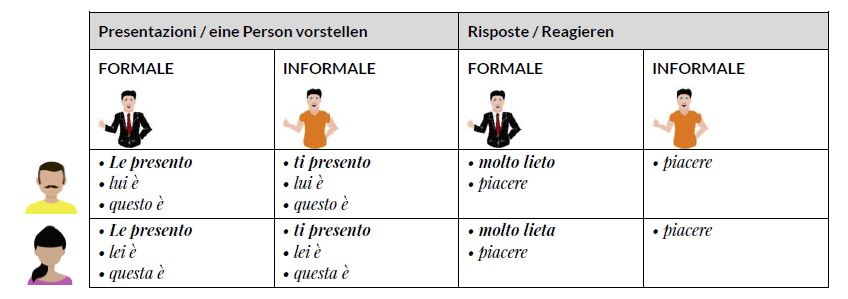
\includegraphics[scale=.8]{images/vorstellen.JPG}
\subsubsection*{Possessivbegleiter}
Die Possessivbegleiter richten sich nach dem Besitz und nicht nach dem Besitzer. Die Possessivbegleiter werden von dem jeweiligen bestimmten Artikel begleitet. il loro /la loro:  das Wort loro ist unveränderlich.\\
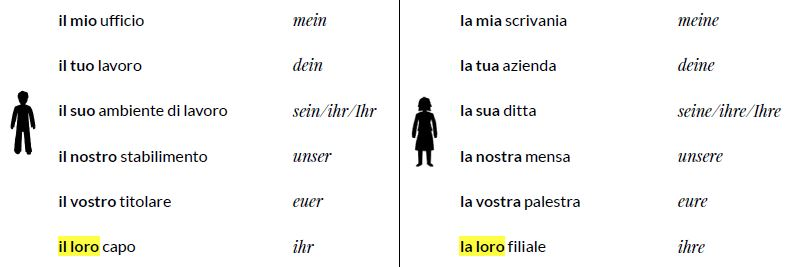
\includegraphics[scale=.8]{images/pbegleiter.JPG}
\\
 Bei Familienbezeichnungen speziell:\\
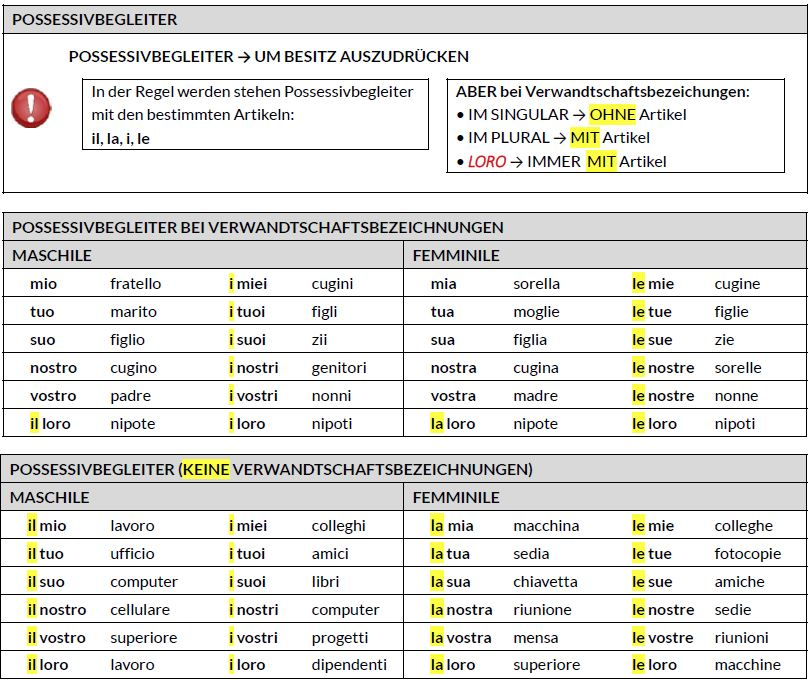
\includegraphics[scale=.7]{images/pbegleiter2.JPG}
\subsubsection*{Über das Wetter sprechen}
Es ist heiss: Fa caldo.\\
Es ist kalt: Fa freddo.\\
Regen: Piove\\
Es schneit: Nevica.\\
Es ist bewölkt: È nuvoloso.
\subsubsection*{Auf dem Bahnhof}
\begin{tabular}{p{4cm}p{4cm}p{4cm}p{4cm}}
Um die Aufmerksamkeit einer Person bitten & Scuci!? & Um eine Notwendigkeit mitzuteilen & Ho bisogno di + SOSTANTIVO / + VERBO\\
Um Miss- oder Unverständnis auszudrücken & Non ho capito bene & Um den Preis der Fahrkarte zu kennen & Quanto costa il biglietto per Roma? \\
Um die Fahrzeit des Zuges zu kennen & A che ora parte il treno? & Um zu wissen, ob sie umsteigen müssen & Devo cambiare? / Dove devo cambiare?\\
Um das Gleis des Zuges zu kennen & Da che binario parte il treno per... & Um Informationen zu bekommen & Vorrei un'informazione.\\
Um Informationen über die Verkehrsverbindungen zu bekommen & Che collegamenti ci sono? & Um sich über das Interessanteste der Region zu informieren & Che cosa c'è da vedere?\\
\end{tabular}
\clearpage
\subsubsection*{Vergangenheit}
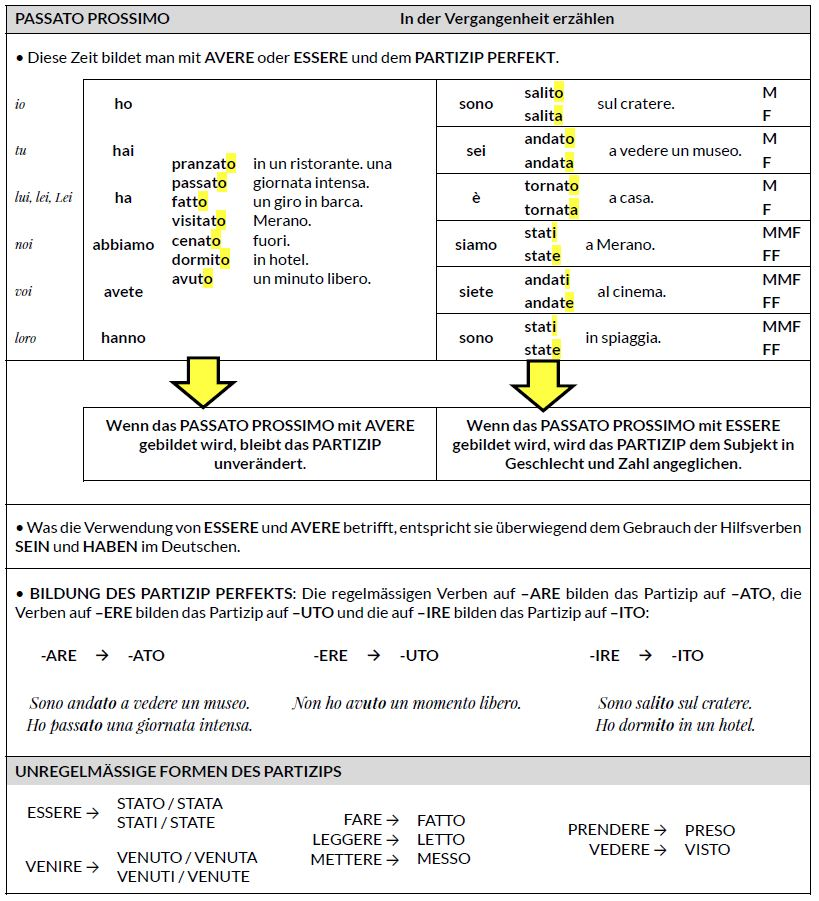
\includegraphics[scale=.8]{images/vergangenheit.JPG}
\subsubsection*{Uhrzeiten}
\begin{tabular}{p{3cm}p{5cm}p{3cm}p{5cm}}
04:10 / 16:10 & Sono le quattro e dieci & 05:15 / 17:15 & Sono le cinque e un quarto\\
09:45 / 21:45 & Sono le dieci meno un quarto / le nove e quarantacinque & 01:00 / 13:00 & È l'una (in punto)\\
08:30 / 20:30 & Sono le otto e mezza / mezzo & 12:00 / 00:00 & È mezzogiorno / mezzanotte\\
\end{tabular}
\end{document}
 